\section{}
\[
H(s)=\frac{s+1}{s+10}\,.
\]
\subsection{Bode-Diagramm}
\begin{center}
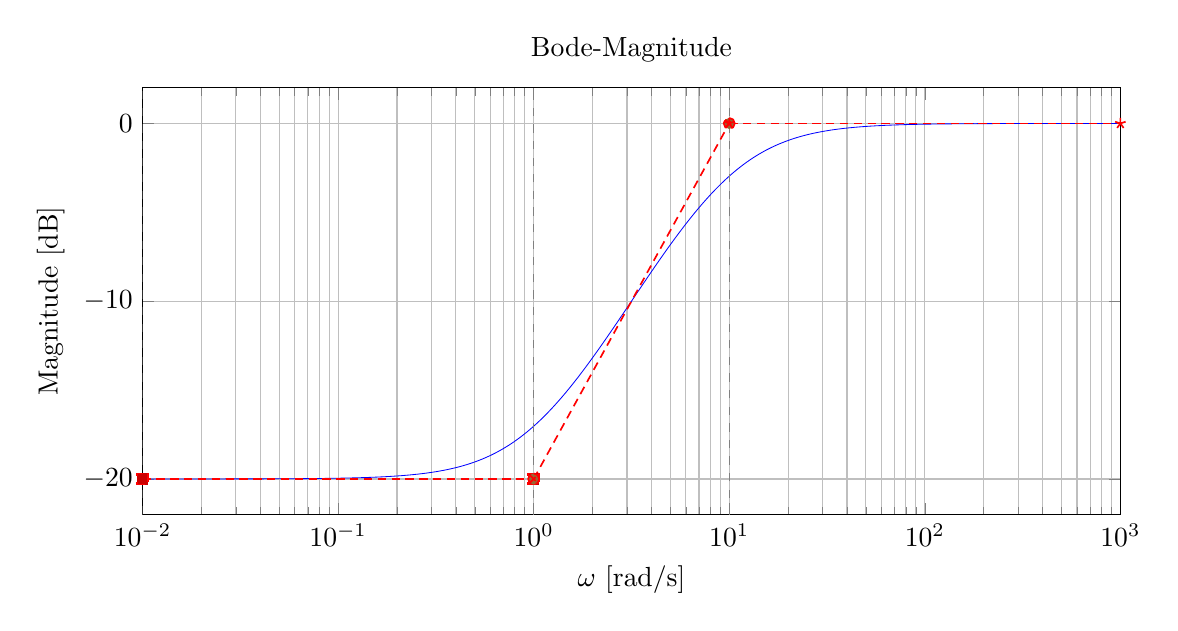
\begin{tikzpicture}
\begin{semilogxaxis}[
  width=14cm,height=7cm,
  xmin=1e-2,xmax=1e3,
  xlabel={$\omega$ [rad/s]},
  ylabel={Magnitude [dB]},
  grid=both,
  ytick distance=10,
  title={Bode-Magnitude}
]
\addplot[
  domain=1e-2:1e3,
  samples=600,
  mark=none,
  line width=0.3pt,
  blue
] {20*ln(sqrt(1 + x^2))/ln(10) - 20*ln(sqrt(100 + x^2))/ln(10)};
\addplot+[domain=1e-2:1,samples=2,dashed,dash pattern=on 3pt off 2pt,line width=0.6pt,red] {-20};
\addplot+[domain=1:1e1,samples=2,dashed,dash pattern=on 3pt off 2pt,line width=0.6pt,red] {-20 + 20*ln(x)/ln(10)};
\addplot+[domain=1e1:1e3,samples=2,dashed,dash pattern=on 3pt off 2pt,line width=0.6pt,red] {0};
\draw[gray,dashed] (rel axis cs:0,0) -- (rel axis cs:0,1);
\draw[gray,dashed] (axis cs:1,\pgfkeysvalueof{/pgfplots/ymin}) -- (axis cs:1,\pgfkeysvalueof{/pgfplots/ymax});
\draw[gray,dashed] (axis cs:10,\pgfkeysvalueof{/pgfplots/ymin}) -- (axis cs:10,\pgfkeysvalueof{/pgfplots/ymax});
\node[gray,anchor=south east] at (axis cs:1,\pgfkeysvalueof{/pgfplots/ymax}) {\scriptsize Nullstelle $\omega_z=1$};
\node[gray,anchor=south east] at (axis cs:10,\pgfkeysvalueof{/pgfplots/ymax}) {\scriptsize Pol $\omega_p=10$};
\end{semilogxaxis}
\end{tikzpicture}
\vspace{6mm}
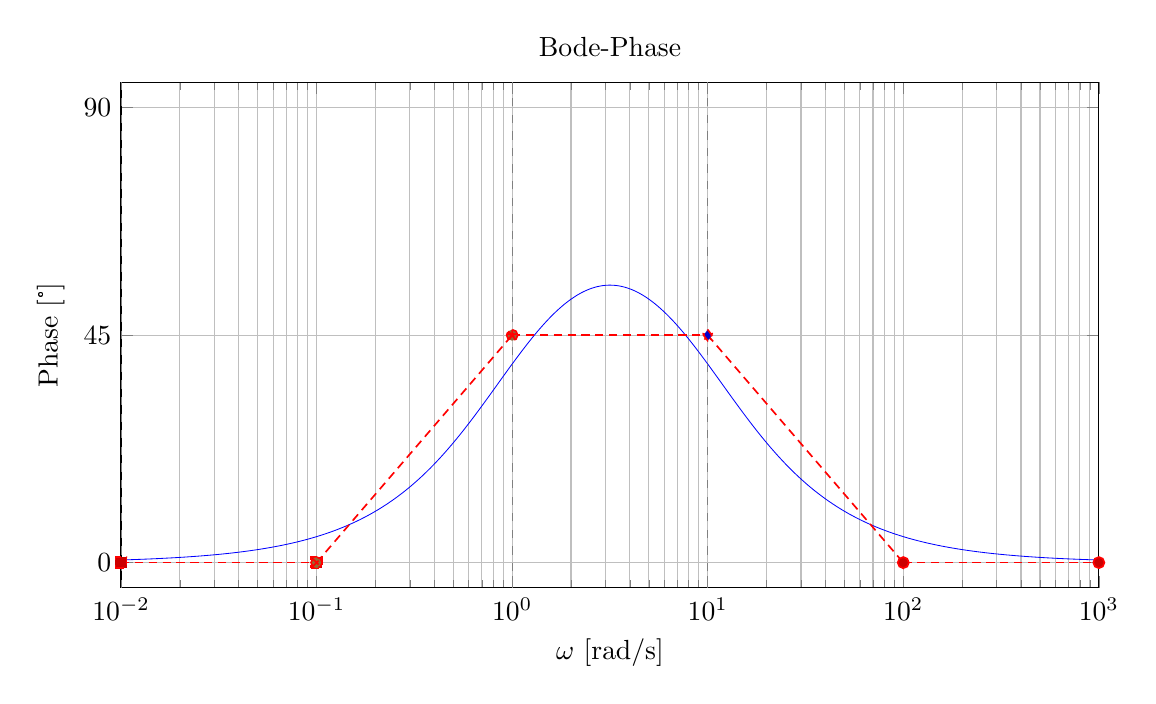
\begin{tikzpicture}
\begin{semilogxaxis}[
  width=14cm,height=8cm,
  xmin=1e-2,xmax=1e3,
  ymin=-5,ymax=95,
  ytick distance=45,
  xlabel={$\omega$ [rad/s]},
  ylabel={Phase [°]},
  grid=both,
  title={Bode-Phase}
]
\addplot[
  domain=1e-2:1e3,
  samples=600,
  mark=none,
  line width=0.3pt,
  blue
] {atan(x) - atan(x/10)};
\addplot+[domain=1e-2:1e-1,samples=2,dashed,dash pattern=on 3pt off 2pt,line width=0.6pt,red] {0};
\addplot+[domain=1e-1:1e0,samples=2,dashed,dash pattern=on 3pt off 2pt,line width=0.6pt,red] {45 + 45*ln(x)/ln(10)};
\addplot+[domain=1e0:1e1,samples=2,dashed,dash pattern=on 3pt off 2pt,line width=0.6pt,red] {45};
\addplot+[domain=1e1:1e2,samples=2,dashed,dash pattern=on 3pt off 2pt,line width=0.6pt,red] {45 - 45*ln(x/10)/ln(10)};
\addplot+[domain=1e2:1e3,samples=2,dashed,dash pattern=on 3pt off 2pt,line width=0.6pt,red] {0};
\draw[gray,dashed] (rel axis cs:0,0) -- (rel axis cs:0,1);
\draw[gray,dashed] (axis cs:1,\pgfkeysvalueof{/pgfplots/ymin}) -- (axis cs:1,\pgfkeysvalueof{/pgfplots/ymax});
\draw[gray,dashed] (axis cs:10,\pgfkeysvalueof{/pgfplots/ymin}) -- (axis cs:10,\pgfkeysvalueof{/pgfplots/ymax});
\node[gray,anchor=south east] at (axis cs:1,\pgfkeysvalueof{/pgfplots/ymax}) {\scriptsize Nullstelle $\omega_z=1$};
\node[gray,anchor=south east] at (axis cs:10,\pgfkeysvalueof{/pgfplots/ymax}) {\scriptsize Pol $\omega_p=10$};
\end{semilogxaxis}
\end{tikzpicture}
\end{center}
\newpage
\subsection{Erklärung}
\vspace{5mm}
\begin{description}[leftmargin=1.2em,labelsep=.6em,font=\bfseries]
\item[Schritt 1] DC-Faktor $\tfrac{1}{10}$: $H(s)=\tfrac{s+1}{s+10}=\tfrac{1+s}{10(1+s/10)}$. Für $\omega\ll1$ dominiert der DC-Anteil: $|H(\j\omega)|\approx\tfrac{1}{10}$, daher Betrag $-20\,\mathrm{dB}$ ohne Startsteigung; Startphase $\approx0^\circ$.
\item[Schritt 2] Nullstelle bei $\omega_z=1\,\mathrm{rad/s}$: ab $\omega=1$ steigt die Magnitude mit $+20\,\mathrm{dB/dec}$; zwischen $\omega_l=0.1$ und $\omega_h=10$ wächst die Phasenbeitrag der Nullstelle näherungsweise linear von $0^\circ$ auf $+90^\circ$ (Geradennäherung: $+45^\circ+45\log_{10}\omega$ in $[0.1,10]$), sodass bei $\omega=1$ etwa $+45^\circ$ erreicht werden.
\item[Schritt 3] Pol bei $\omega_p=10\,\mathrm{rad/s}$: ab $\omega=10$ kommt ein Steigungswechsel von $-20\,\mathrm{dB/dec}$ hinzu; dadurch wird die Gesamtslope wieder $0\,\mathrm{dB/dec}$ und der Betrag konvergiert gegen $0\,\mathrm{dB}$ für $\omega\gg10$. Der Pol führt in $[1,100]$ zu einer Phasenabnahme um $90^\circ$ (Geradennäherung: $+45^\circ-45\log_{10}(\omega/10)$), sodass die Gesamtphase für $\omega\gg100$ wieder gegen $0^\circ$ fällt. Das Zwischenband $1\le\omega\le10$ ist somit nahezu phasenflach bei $\approx+45^\circ$ und weist eine Betrags-Slope von $+20\,\mathrm{dB/dec}$ auf.
\end{description}

\vspace{0.5cm}
\medskip
\noindent\textbf{Stückweise Näherung}
\[
|H(\j\omega)|_{\mathrm{dB}}\approx
\begin{cases}
-20,& \omega\ll1,\\[4pt]
-20+20\log_{10}\omega,& 1\ll\omega\ll10,\\[4pt]
0,& \omega\gg10,
\end{cases}
\qquad
\]
\newpage